\documentclass[10pt,fancyhdr,graybox, envcountchap,oribibl,twoside]{svmono}

\usepackage[UTF8]{ctex}
%\usepackage{ifxetex}

%153  body={120mm,195mm}
\usepackage[centering,paperwidth=190mm,paperheight=235mm,left=18mm,marginparsep=3mm,marginparwidth=30mm,textwidth=120mm,height=195mm]{geometry}

%------------------------------------

\usepackage{fancyhdr}
\pagestyle{fancy}
\renewcommand{\sectionmark}[1]{\markright{\thesection.\ #1}}
\renewcommand{\chaptermark}[1]{\markboth{\thechapter.\ #1}{}}
\fancyhead[LO]{\rightmark}
\fancyhead[RO]{\thepage}
\fancyhead[LE]{\thepage}
\fancyhead[RE]{\leftmark}
\fancyfoot[C]{}
\addtolength\headwidth{33mm}

%\usepackage[width=153mm,outermargin=-33mm]{fullwidth}
\usepackage[outermargin=-33mm, innermargin=0.0mm,width=153mm]{fullwidth}


%------------------------------------

\usepackage{multicol}
\newcommand{\multicolumnmtc}{2}

\usepackage[tight]{minitoc}
\setcounter{minitocdepth}{1}
\setlength{\mtcindent}{0pt}
\mtcsetpagenumbers{minitoc}{off}
\def\mtctitle{}
\mtcsetformat{minitoc}{tocrightmargin}{2.55em plus 1fil}
\makeatletter
 \let\SV@mtc@verse\mtc@verse
 \let\SV@endmtc@verse\endmtc@verse
 \def\mtc@verse#1{\SV@mtc@verse#1\removelastskip%
 \begin{multicols}{\multicolumnmtc}\raggedcolumns\leavevmode\unskip  \vskip -1.0ex \vskip -1\baselineskip}
 \def\endmtc@verse{\end{multicols}\SV@endmtc@verse}
\makeatother

%------------------------------------

\usepackage[utf8]{inputenc}
\usepackage{tcolorbox}
\usepackage{titlesec} 
\titleformat{\chapter} % command
[block] % shape
{} % format
{\begin{tcolorbox}[height=2.5cm,width=2.5cm,colback=white,boxrule=1.6mm,arc=0mm,valign=center,halign=center] \Huge\thechapter\end{tcolorbox}} % label
{0.0ex} % sep
{
    \raggedright\bfseries\Huge\itshape
} % before-code
[
\vspace{2.5ex}%
] %

%------------------------------------

\usepackage{mathptmx}        % selects Times Roman as basic font
\usepackage{helvet}          % selects Helvetica as sans-serif font
\usepackage{courier}         % selects Courier as typewriter font
%\usepackage{type1cm}        % activate if the above 3 fonts are 
                             % not available on your system

\usepackage{makeidx}         % allows index generation
\usepackage{graphicx}        % standard LaTeX graphics tool
                             % when including figure files
\usepackage{multicol}        % used for the two-column index
\usepackage[bottom]{footmisc}% places footnotes at page bottom

% see the list of further useful packages in the Reference Guide




\usepackage{amsmath}
\usepackage{caption}
\usepackage{subcaption}
\captionsetup{compatibility=false}
\usepackage{array}
\usepackage{listings}
\usepackage{url}
\usepackage{color}


\usepackage{calc}
\usepackage[strict]{changepage}

\newlength\mymargin
\setlength{\mymargin}{\marginparwidth+\marginparsep}
\newlength\mylength
\setlength{\mylength}{\textwidth +\mymargin}




\makeindex             % used for the subject index
   


\begin{document}

然而事情并不这么简单,对于给定分辨率的“屏幕”,它的每一个像素点总是有一个尺寸大小的。而对于每个像素,我们通常取其从摄像机发出穿过该像素中心点的方向对场景进行采样,如果一个像素的中心点被三角形覆盖,则整个像素被填充一个单一的颜色,否则即使该像素有小部分区域被覆盖,它也不会被填充任何颜色,这使得三角形的边缘出现锯齿(Aliasing\index{Aliasing}),如图\ref{f:intro-aliasing-triangle}所示,而尝试避免或者减少这种锯齿的技术称为反锯齿(Anti-aliasing\index{Anti-aliasing})技术。

\begin{figure}
\sidecaption
	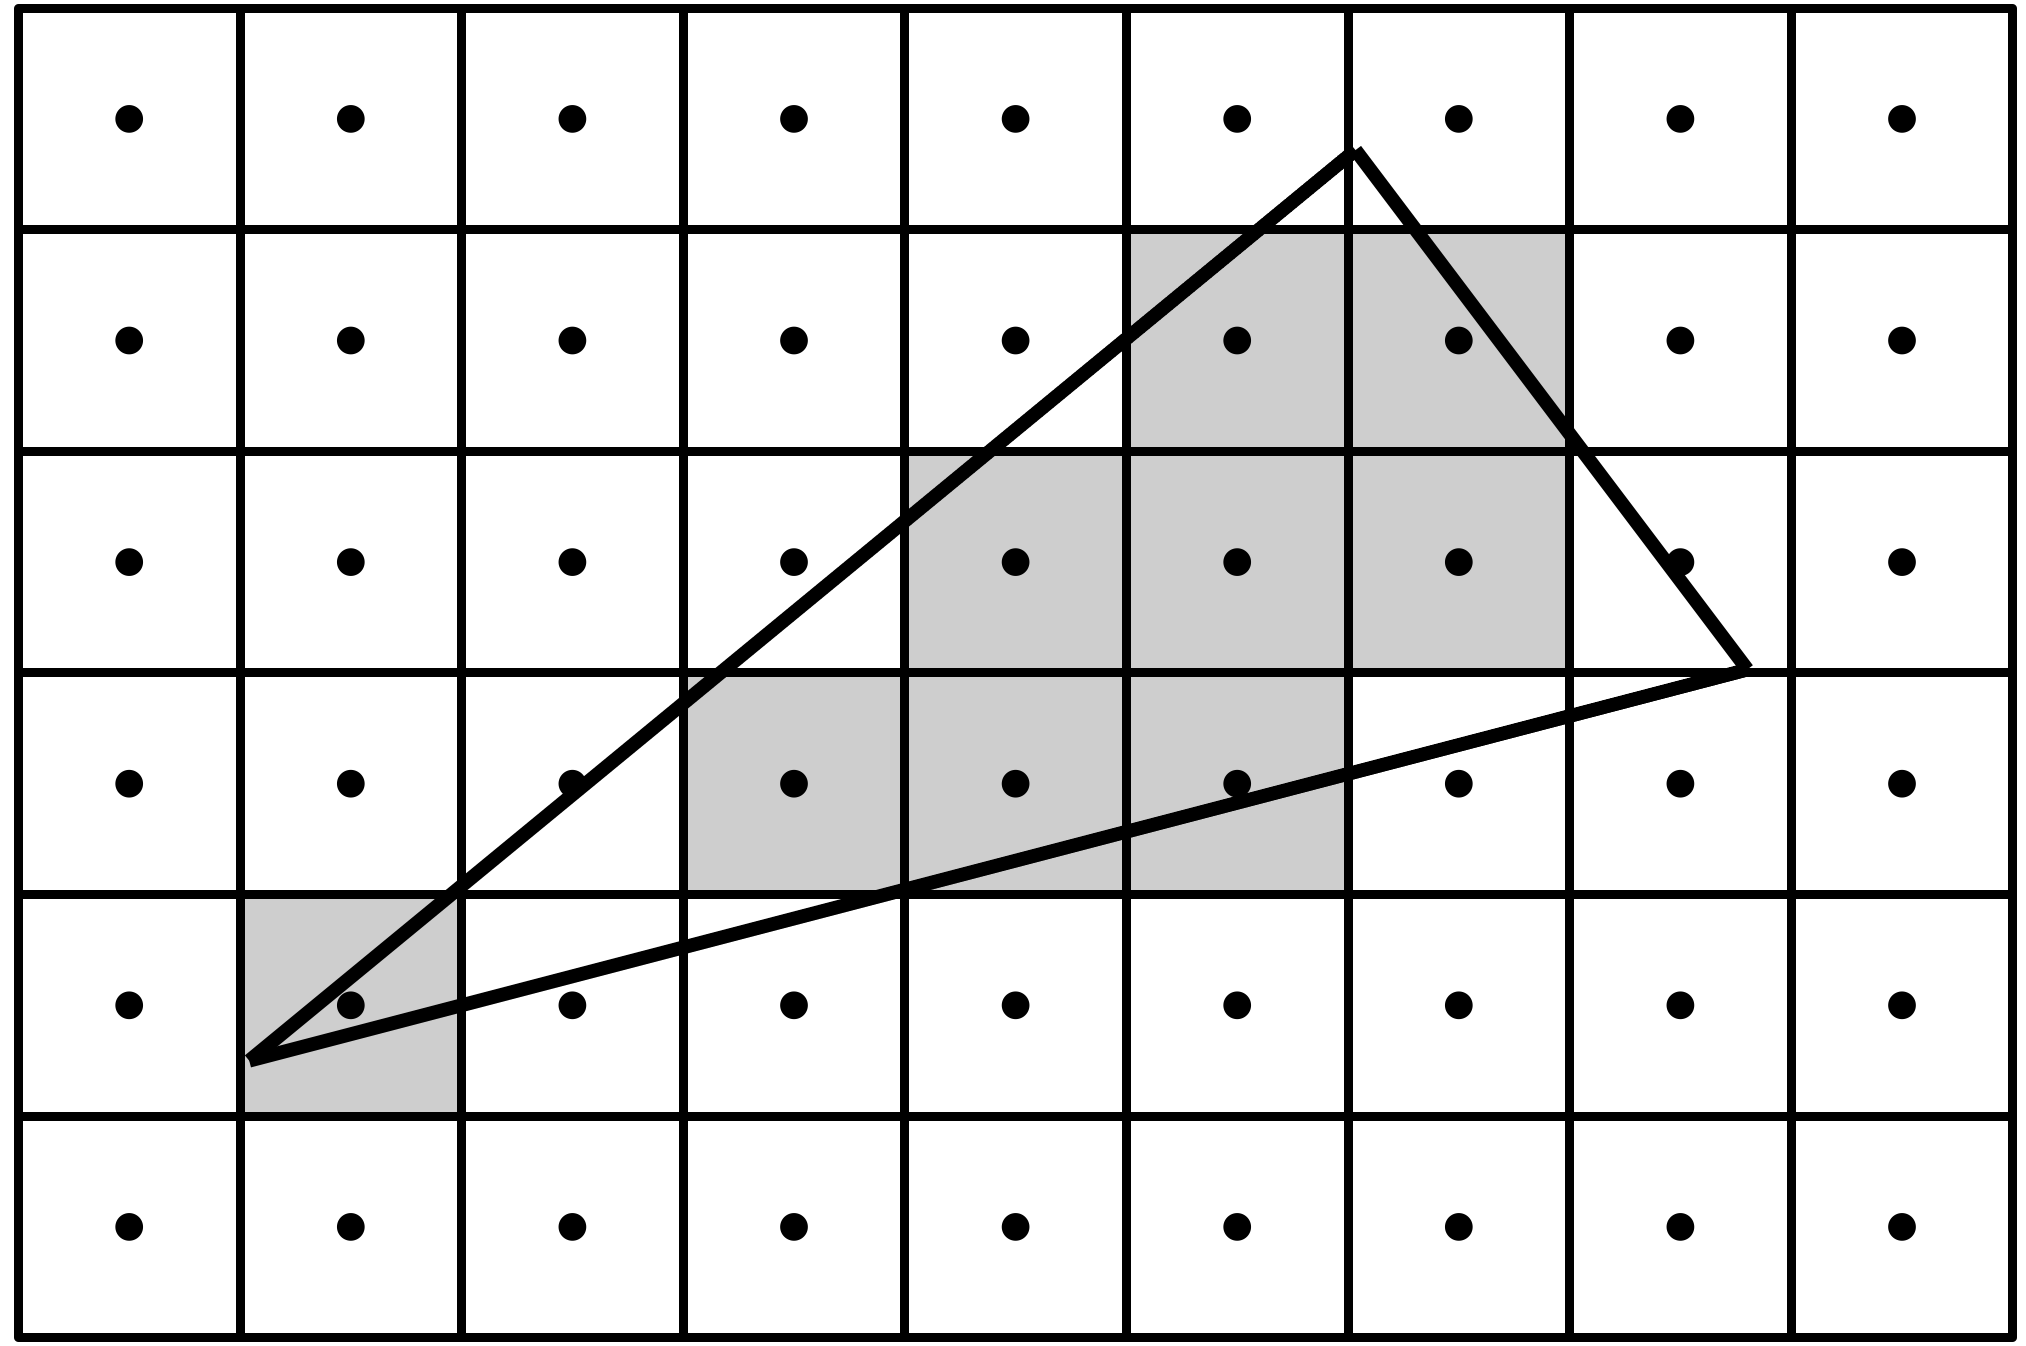
\includegraphics[width=0.5\textwidth]{figures/intro/aliasing-triangle}
	\caption{光栅化技术通过测试几何图形对像素中心点的覆盖来决定是否对该像素点着色,这造成在几何图形的边缘出现锯齿现象。}
	\label{f:intro-aliasing-triangle}
\end{figure}

用数学理论来解释和解决这种缺陷,涉及到数字信号处理的一些理论,如采样,重建,过滤等。这些技术的学习不仅有助于理解渲染过程中数字图像的生成过程,它也是计算机图形学的重点内容,例如着色器中对纹理的采样,Post Processing中很多都涉及到过滤技术等等。接下来,我们讨论关于数字信号处理的一些理论,并解释这些理论怎样被用在计算机图形学中。





\subsection{采样和过滤技术}
3D图像的生成本质上是一个对各种连续函数(如几何图形,高光分布函数等)采样,转化为对应的一个离散函数(以有限分辨率表示的一个二维图像)的过程。3D渲染的大部分采样发生在光栅化阶段,或者其他由光栅化导致的采样,例如图\ref{f:intro-aliasing-triangle}中,三角形两个顶点之间的边是连续的,但是被光栅化过程采样为离散的像素值。

\begin{figure}
	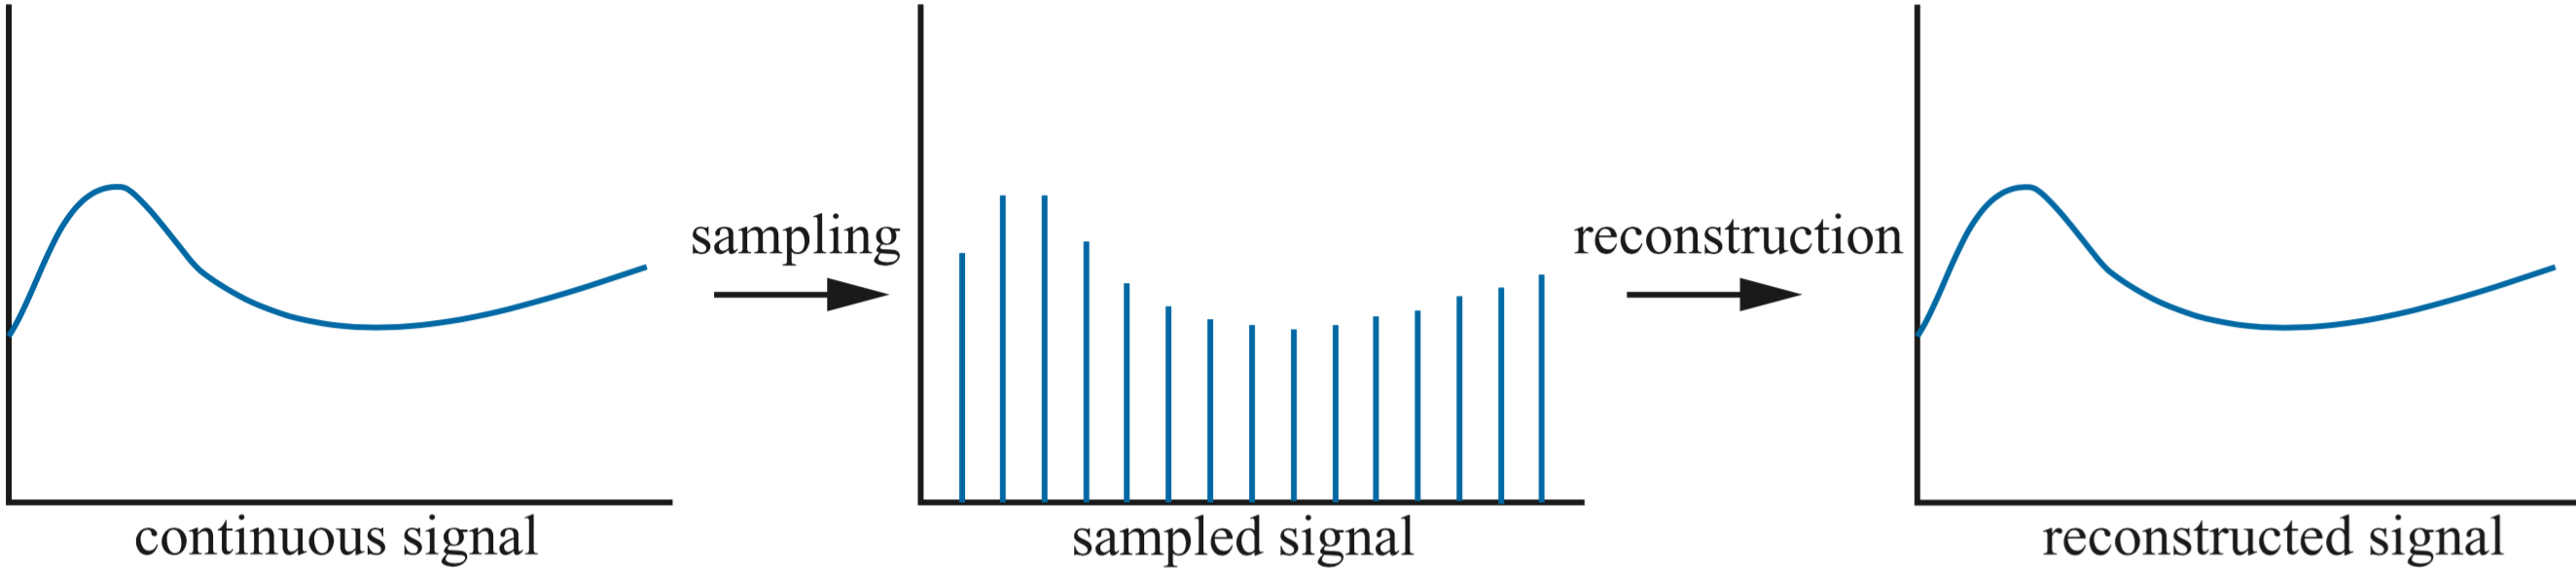
\includegraphics[width=1.0\textwidth]{figures/intro/signal-processing}
	\caption{一个连续的信号被采样为离散的信号,然后通过重建还原为接近原连续信号的连续信号。}
	\label{f:intro-signal-processing}
\end{figure}

在数字信号处理(Digital Signal Processing\index{Digital Signal Processing})中,术语采样(Sampling\index{Sampling})的目的是将连续的信号表述为离散的信号,在采样的过程中,其中的一些信息会丢失;为了重建(Reconstruction\index{Reconstruction})原始连续信号,则需要对离散信号使用过滤(Filtering\index{Filtering})技术来还原原始离散信号。



\subsubsection{Sampling}\index{Sampling}
关于采样的理论非常复杂,它涉及到傅立叶变换,积分,级数等数学知识以及像频率域等滤波相关的概念。然而理解采样相关知识是理解锯齿相关知识的重要理论基础,而且在图形学的其他一些地方也会涉及到这些知识,例如在光线追踪技术中就会大量涉及脉冲函数;理解傅立叶变换也有助于理解后面的Spherical harmonics函数等。但本节不会严格地推导和讨论傅立叶相关的知识,而只是使用一些结论让读者比较容易地理解采样相关的概念及逻辑,关于更多关于数字图像处理的理论知识,可以参考\cite{b:DigitalImageProcessing}。

\begin{figure}
\begin{fullwidth}
	\begin{subfigure}[b]{0.33\textwidth}
		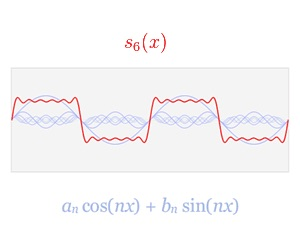
\includegraphics[width=1.\textwidth]{figures/intro/fourier-1}
	\end{subfigure}
	\begin{subfigure}[b]{0.33\textwidth}
		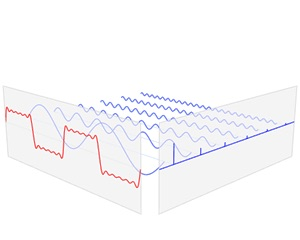
\includegraphics[width=1.\textwidth]{figures/intro/fourier-2}
	\end{subfigure}
	\begin{subfigure}[b]{0.33\textwidth}
		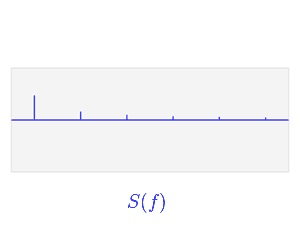
\includegraphics[width=1.\textwidth]{figures/intro/fourier-3}
	\end{subfigure}
\caption{傅立叶变换将函数由时间域(或空间域)变换到频率域(图片来自Wikipedia)。}
\label{f:intro-fourier}
\end{fullwidth}
\end{figure}


法国数学家傅立叶( Jean Baptiste Joseph Fourier)于1807年在他的《热分析理论》一书中指出,任何周期函数都可以表示为不同频率的正弦和(或余弦和)的形式,每个正弦项(或余弦项)乘以不同的系数,称该和为傅立叶级数。例如具有周期$T$的连续变量$t$的周期函数$f(t)$的傅立叶级数为:

\begin{equation}
	f(t)=\sum^{\infty}_{n=-\infty}c_n e^{j\frac{2\pi n}{T}t}
\end{equation}

其中:

\begin{equation}
	c_n=\frac{1}{T}\int^{T/2}_{-T/2}f(t)e^{-j\frac{2\pi n}{T}t}dt, n=0,n=\pm 1,n=\pm 2,\cdots
\end{equation}

实际上非周期(但该曲线下的面积是有限的)也可以用正弦和(或余弦和)乘以一个加权函数(而非一个常数)的积分来表示,在这种情况下的公式就是傅立叶变换。用$F(\mu)$表示连续变量$t$的连续函数$f(t)$的傅立叶变换,则:

\begin{equation}\label{eq:intro-fourier}
	F(\mu)=\int^{\infty}_{-\infty}f(t)e^{-j2\pi\mu t}dt
\end{equation}

相反,给定$F(\mu)$,通过傅立叶反变换可以获得$f(t)$:

\begin{equation}
	f(t)=\int^{\infty}_{-\infty}F(\mu)e^{-j2\pi\mu t}d\mu
\end{equation}

利用欧拉公式\footnote{$e^{j\theta}=cos\theta +jsin\theta$},可以把傅立叶变换公式\ref{eq:intro-fourier}表示为:

\begin{equation}
	F(\mu)=\int^{\infty}_{-\infty}f(t)[cos(2\pi\mu t)-jsin(2\pi\mu t)]dt
\end{equation}

我们看到,由于变量$t$被积分后只剩下$\mu$,而$\mu$表示正弦项或余弦项的频率,所以傅立叶变换$F(\mu)$的作用域是频率域。频率变量$\mu$的单位取决于$t$的单位,例如,如果$t$表示单位为秒的时间,则$\mu$的单位为周/秒,如果$t$表示单位为米的时间,则$\mu$的单位为周/米。在图\ref{f:intro-fourier}中可以看到这种作用域的转化,这个频率作用域将用于后面对信号采样的质量判定。



\begin{figure}
\begin{fullwidth}
	\begin{subfigure}[b]{0.33\textwidth}
		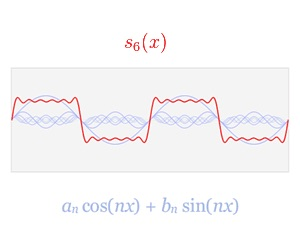
\includegraphics[width=1.\textwidth]{figures/intro/fourier-1}
	\end{subfigure}
	\begin{subfigure}[b]{0.33\textwidth}
		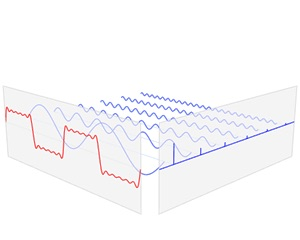
\includegraphics[width=1.\textwidth]{figures/intro/fourier-2}
	\end{subfigure}
	\begin{subfigure}[b]{0.33\textwidth}
		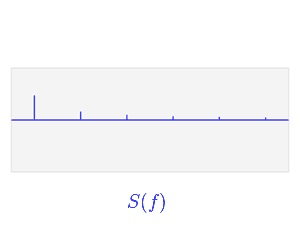
\includegraphics[width=1.\textwidth]{figures/intro/fourier-3}
	\end{subfigure}
\caption{傅立叶变换将函数由时间域(或空间域)变换到频率域(图片来自Wikipedia)。}
\label{f:intro-fourier}
\end{fullwidth}
\end{figure}







\end{document}